\documentclass[border=5pt]{standalone}
\usepackage{tikz}
\usetikzlibrary{arrows.meta,decorations.pathmorphing,calc}
\definecolor{boxgray}{RGB}{237,237,237}
\begin{document}
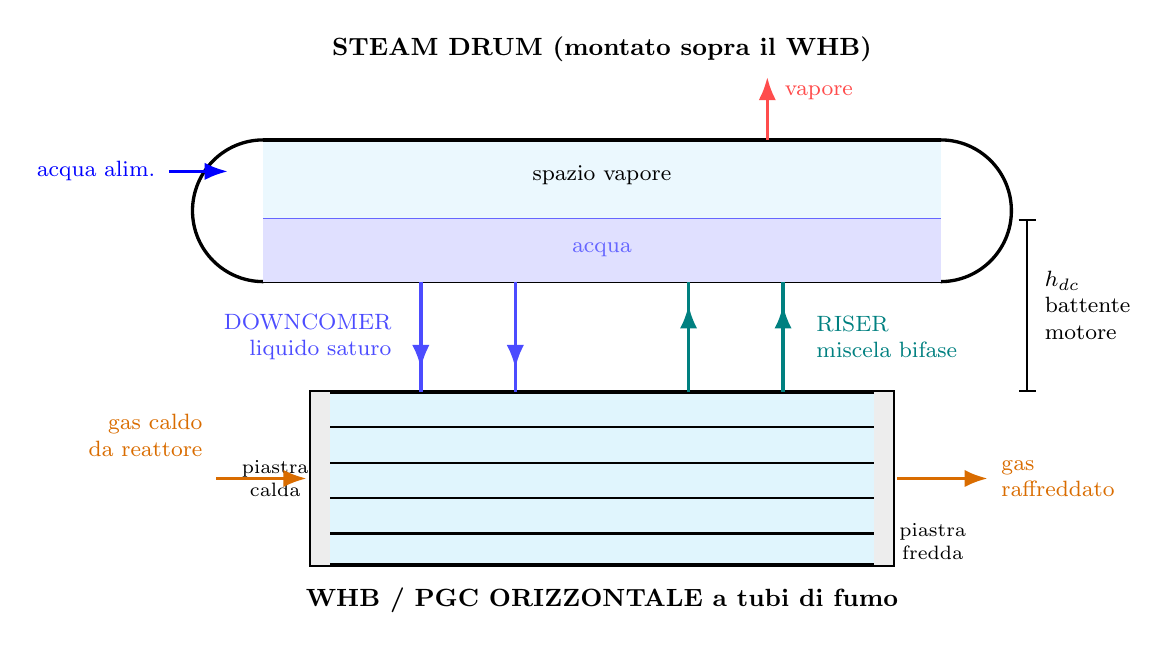
\begin{tikzpicture}[font=\footnotesize]

% ===== STEAM DRUM (above) =====
\fill[cyan!8] (1.2,4.2) rectangle (9.8,6.0);
\draw[very thick] (1.2,4.2) -- (9.8,4.2);
\draw[very thick] (1.2,6.0) -- (9.8,6.0);
\draw[very thick] (1.2,4.2) arc (-90:-270:0.9);
\draw[very thick] (9.8,4.2) arc (-90:90:0.9);
% water level
\draw[thick,blue!60] (1.2,5.0) -- (9.8,5.0);
\fill[blue!12] (1.2,4.2) rectangle (9.8,5.0);
\node[blue!60] at (5.5,4.6) {acqua};
\node at (5.5,5.55) {spazio vapore};
\node[font=\small\bfseries] at (5.5,7.15) {STEAM DRUM (montato sopra il WHB)};
% steam outlet
\draw[-{Latex},very thick,red!70] (7.6,6.0) -- (7.6,6.8);
\node[red!70,anchor=west] at (7.7,6.6) {vapore};
% feedwater
\draw[-{Latex},very thick,blue] (0.0,5.6) -- (0.75,5.6);
\node[blue,anchor=east] at (-0.05,5.6) {acqua alim.};

% ===== WHB (below, horizontal) =====
\fill[cyan!12] (1.8,0.6) rectangle (9.2,2.8);
\draw[very thick] (1.8,0.6) rectangle (9.2,2.8);
\fill[boxgray] (1.8,0.6) rectangle (2.05,2.8);
\fill[boxgray] (8.95,0.6) rectangle (9.2,2.8);
\node[font=\scriptsize,align=center] at (1.35,1.7) {piastra\\calda};
\node[font=\scriptsize,align=center] at (9.7,0.9) {piastra\\fredda};
\foreach \y in {1.0,1.45,1.9,2.35}{
  \draw[thick] (2.05,\y) -- (8.95,\y);
}
\node[font=\small\bfseries] at (5.5,0.15) {WHB / PGC ORIZZONTALE a tubi di fumo};
% gas flow
\draw[-{Latex},very thick,orange!85!black] (0.6,1.7) -- (1.75,1.7);
\node[orange!85!black,anchor=east,align=right] at (0.55,2.25) {gas caldo\\da reattore};
\draw[-{Latex},very thick,orange!85!black] (9.25,1.7) -- (10.4,1.7);
\node[orange!85!black,anchor=west,align=left] at (10.45,1.7) {gas\\raffreddato};

% ===== RISERS (up, right side) =====
\foreach \x in {6.6,7.8}{
  \draw[very thick,teal] (\x,2.8) -- (\x,4.2);
  \draw[-{Latex},very thick,teal] (\x,3.1) -- (\x,3.9);
}
\node[teal,anchor=west,align=left] at (8.1,3.5) {RISER\\ miscela bifase};

% ===== DOWNCOMERS (down, left side) =====
\foreach \x in {3.2,4.4}{
  \draw[very thick,blue!70] (\x,4.2) -- (\x,2.8);
  \draw[-{Latex},very thick,blue!70] (\x,3.9) -- (\x,3.1);
}
\node[blue!70,anchor=east,align=right] at (2.95,3.5) {DOWNCOMER\\ liquido saturo};

% height annotation
\draw[|-|,thick] (10.9,2.8) -- (10.9,5.0);
\node[anchor=west,align=left] at (11.0,3.9) {$h_{dc}$\\ battente\\ motore};

\end{tikzpicture}
\end{document}
